%%% fs-run-time-impl Implementation
\label{fs-impl}

\FlameStream\ is implemented in Java, using Akka framework for messaging and Apache Zookeeper for cluster state management.

\subsection{Ordering model}
The meta-information of data item is implemented as a tuple of a {\it global time}, a {\it trace}, {\it child ids} and a {\it tombstone flag}.

\[Meta := (GlobalTime, ChildIds[], Trace, IsTombstone)\]

Global time is assigned to data item once the item enters the system. It is a pair of logical time and the identifier of the front. The identifier is used to resolve time collisions within different fronts. It is important to notice that we do not rely on any clock synchronization between nodes. The only implication of the clock skew is the system degradation regarding latency: 1 ms of the fronts clock difference appends 1 ms to minimal latency.

Each map operation can produce multiple items from one.  An ordinal number, {\it child id}, is stored in the meta information to differentiate them. {\it ChildIds} is an array of child ids, that corresponds to all visited map operations.

The global time and child ids are enough to uniquely identify data item within stream if all processing is done in-order. If there are any grouping repairs happened during processing, multiple items with the same global time and child ids exist in the stream. 

To match tombstone item with an invalidated item, there is {\it Trace} value stored in the meta-information. The unique random 64-bit identifier is assigned to each physical operation. The trace is a xor of all operations' ids visited by item so far. Invalid item and the corresponding tombstone go along the same path, because they have the same payload and the balancing functions are deterministic, so they have the same trace values.

Metas are compared lexicographically and this order is in line with the \FlameStream's ordering model.

Figure~\ref{logical-graph-ops-figure} shows the topology of each operation and how it affects the meta. Grouping and merge operations update trace of the data item by xoring initial trace with its physical id. Map and broadcast apply the same update, but also append child id for each output item.

\begin{figure}[ht]
  \centering
  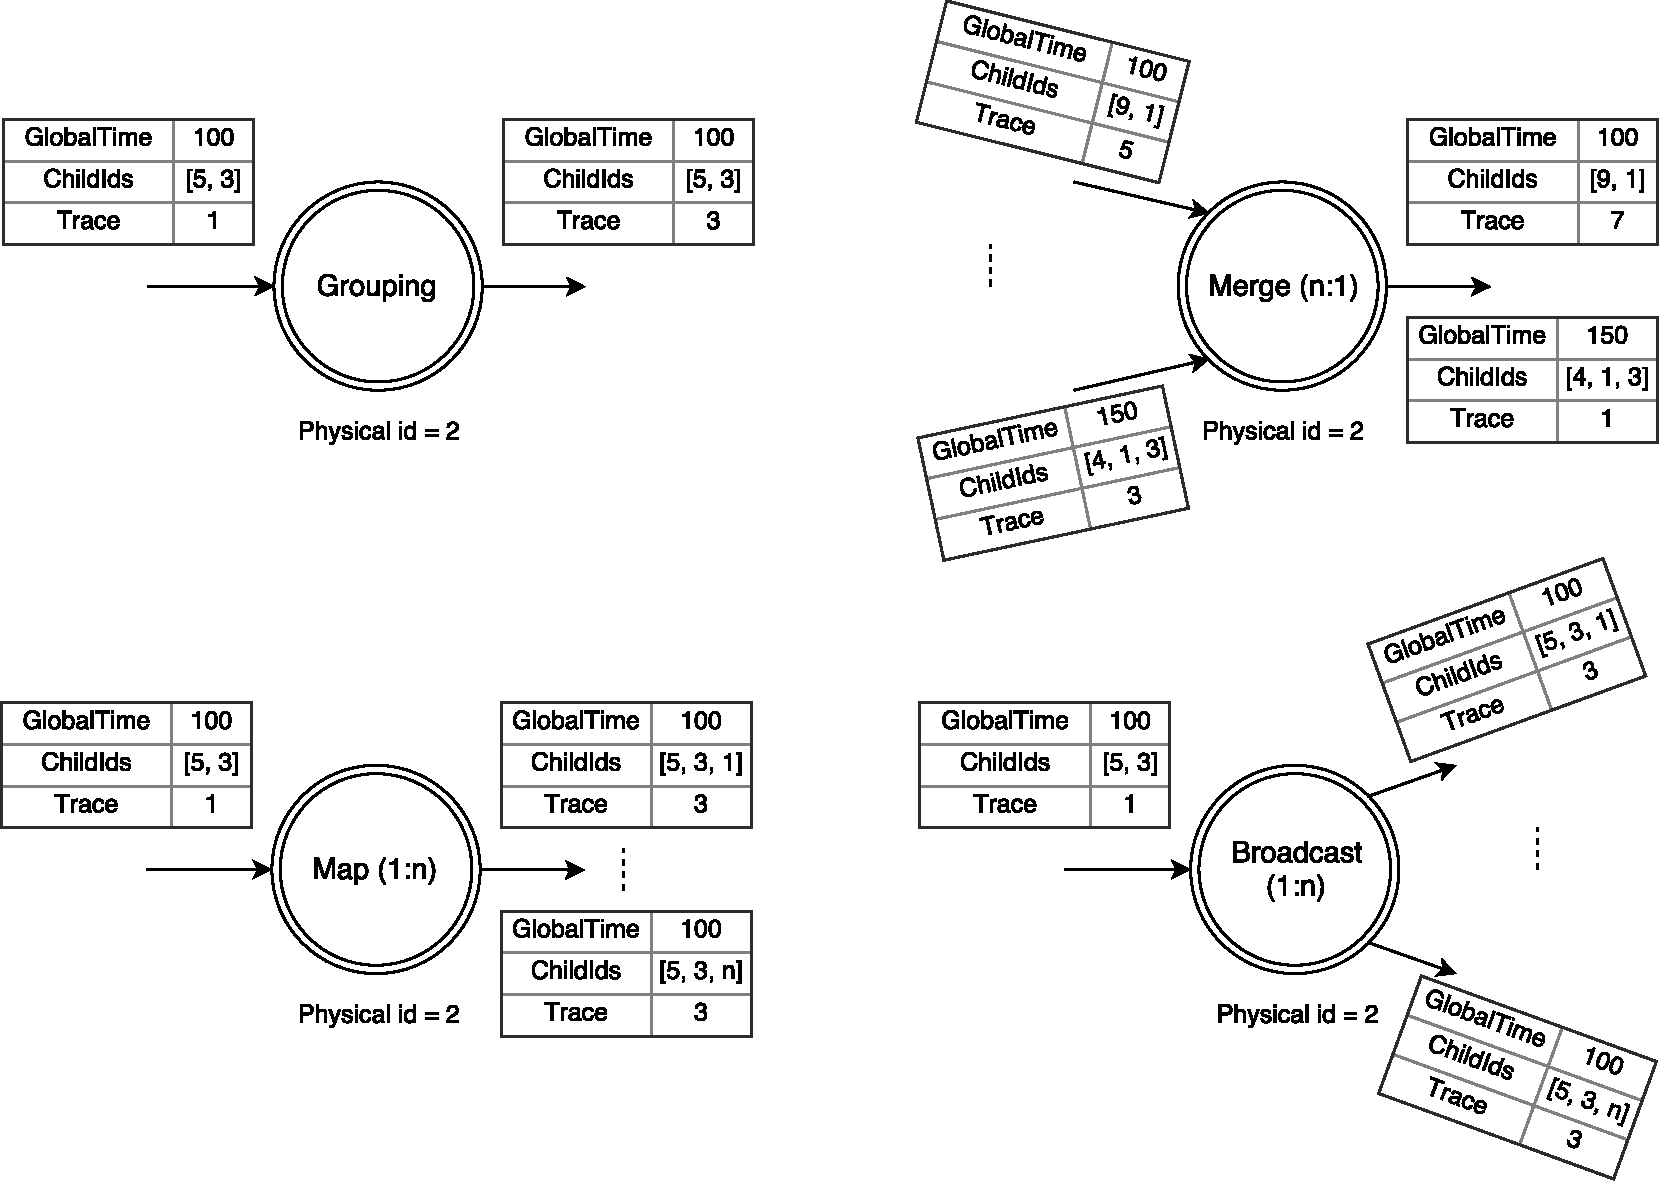
\includegraphics[width=\linewidth]{pics/operations}
  \caption{The topology of each operation and how it affects the meta}
  \label {logical-graph-ops-figure}
\end{figure}

\label{mininal-time}

\subsection{Minimal time within stream}

To release an item from the barrier we need to ensure that there are no in-flight tombstones for that item. 

\newtheorem{minimal-time-claim}{Lemma}

\begin{minimal-time-claim}
  If data item {\it D} has global time {\it GT} greater than the global time of each in-flight element, then all tombstones for that item had already arrived at the barrier.
\end{minimal-time-claim}

\begin{proof}
  Let $D_{tomb}$ be an in-flight tombstone for {\it D}. According to the definition of the tombstone item, $D_{tomb}$ and {\it D} has the same global time {\it GT}. We assumed that there are no in-flight element with the global time equal to {\it GT}. Contradiction.
  
  New tombstones for {\it D} cannot be generated because items with global time greater than {\it GT} cannot trigger repair that affects {\it D}.

  This implies that if the stream does not contain items with the global time less than or equal to {\it GT}, then all tombstones for {\it D} had already arrived at the barrier. 
\end{proof}

Therefore, to output an item from the barrier, we should ensure that there are no items in the stream with the global time less than or equal to the global time of this item.

To track the global time of in-flight items we adopt an idea of {\it acker task} inspired by Apache Storm~\cite{apache:storm}. Acker tracks data items using a checksum hash. When the item is sent or received by an operation, its global time and checksum are sent to the acker. This message is called {\it ack}. Acker groups acks by a global time and xors received checksum hashes. When an item is sent and later received by the next operation, xoring corresponding {\it XOR}s would yield zero.

Acks are overlapped to nullify {\it XOR} only when an item arrives at the barrier. That is, ack for receive is sent only after both processing and the ack sending for the transformed item, as illustrated in Figure~\ref{acker}. This technique guarantees that the {\it XOR} for some global time is equal to zero only if there are no in-flight elements with such global time.

\begin{figure}[ht]
  \centering
  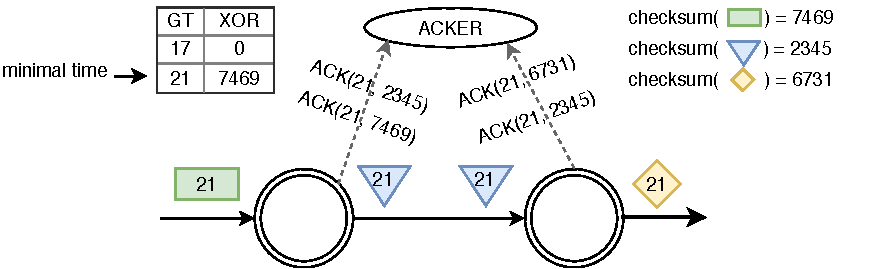
\includegraphics[width=0.8\textwidth]{pics/acker}
  \caption{The example of tracking minimal time using acker}
  \label {acker}
\end{figure}

The minimal time within a stream is the minimal global time with non-zero {\it XOR}. On minimal time changes, acker broadcasts the {\it new minimal time notification}. Therefore, the barrier can release elements with global time {\it GT} once it received notification with time greater than {\it GT}.

To ensure that no fronts can generate item with the specific timestamp, each front periodically sends to acker special message called {\it heartbeat}, which promises that front will not generate items with a timestamp lower than the reported. The value in the ack table can become zero only after the corresponding heartbeat arrives.

The proposed mechanism could be isolated by hash range. This change allows us releasing from barriers on different workers independently. This feature is also known as early key availability.
